\documentclass[main.tex]{subfiles}
\begin{document}
\begin{enumerate}

\subsection*{Section 4 Electromagnetics, Radiation Systems \& Microwave Engineering}

\item [10.] The magnetic field of a particular mode in a parallel-plate air waveguide with a plate separation of 2.5 cm is given by
$$H_{z}(x, y)=C e^{-j 640 \pi x / 3} \cos (160 \pi y)$$
where x and y are both in meters.
    
    \begin{enumerate}
        \item \textbf{Q.} Is this a TE\textsubscript{n} or TM\textsubscript{n} mode? What is n? Is it a propagating or non-propagating mode? \textbf{A.} Consider the propagation direction is $x$ instead of $z$. The general form of a magnetic field for Transverse Magnetic (TM) mode is
        
        $$
        H z(x, y)=C_1 e^{-\gamma^x} \cos \left(\frac{m \pi}{a}\right) y.
        $$
        
        By comparing equations this is $\mathrm{TM_n}$ mode

        $$
        \begin{aligned}
        \gamma &= \frac{j 640 \pi}{3} \mathrm{rad}/\mathrm{m}\\
        \frac{m \pi}{a} &= 160 \pi
        \end{aligned}
        $$
        
        Here $a=2.5 \mathrm{~cm}=2.5 \times 10^{-2} \mathrm{m}$

        $$
        \begin{aligned}
        \frac{m \pi}{2.5 \times 10^{-2}} &= 160 \pi \\
        m &= 4
        \end{aligned}
        $$

        Therefore, it is $\mathrm{TM_4}$ mode. The constant $\gamma$ is purely imaginary therefore it is a propagating mode.
        
        \item \textbf{Q.} What is the operating frequency? \textbf{A.}

        $$
        \begin{aligned}
        b_{c2} &= \frac{m c}{2 a} \\
        &= \frac{4 \times 3 \times 10^8}{2 \times 2.5 \times 10^{-2}} \\
        &= 24 \mathrm{GHz} \\
        r_2 = \alpha_2 = \frac{640}{3} &= \beta \sqrt{\left(\frac{b c_2}{f}\right)^2-1} \\
        \frac{640}{3} &= \frac{2 \pi f}{c} \sqrt{\left(\frac{b c_2}{b}\right)^2-1}
        \end{aligned}
        $$
        squaring on both sides,
        $$
        \left(\frac{640}{3}\right)^2=\frac{4 \pi^2 f^2}{c^2}\left[\left(\frac{f c_2}{f}\right)-1\right]
        $$
        
        $$
        \begin{aligned}
        \left(\frac{640}{3}\right)^2 & =\frac{4 \pi^2 f^2}{\left(3 \times 10^8\right)^2}\left[\frac{24 \times 10^9}{f}-1\right] \\
        1.637 \times 10^{20} & =\frac{f^2}{f}\left[24 \times 10^9-1\right] \\
        1.037 \times 10^{20} & =\left(24 \times 10^9\right) 6-f \\
        1.037 \times 10^{20} & =\left(24 \times 10^9\right) f \\
        f & =\frac{1.037 \times 10^{20}}{24 \times 10^9} \\
        f & =4.32 \mathrm{GHz}
        \end{aligned}
        $$
        
        \item \textbf{Q.} Find the corresponding electric field. \textbf{A.}

        $$
        H(x, y)=\frac{E(x, y)}{\eta}
        $$
        
        where $\eta$ is the intrinsic impedance, 
        
        $$
        \begin{aligned}
        \eta &= 120 \pi=377 \Omega \\
        E(x, y) &= 377 C_1 \text { exp }\left(-j \frac{640 \pi}{3}\right) x \cos (160 \pi y) \hat{x}
        \end{aligned}
        $$
        
    \end{enumerate}
    
\item [11.] An electromagnetic field in free space, $\mu_{0}=4 \pi \times 10^{-7}$ henry/meter, $\varepsilon_0 = 8.85 \times 10^{-12}$ farads/meter, is specified as by the vector phasor 

$$\underline{E}(\underline{r})=\underline{E}_{0} \varepsilon^{-j \underline{k} \underline{g} \underline{r}}$$

where $\underline{E}_{0}=\hat{x}$ the unit vector in the x direction of a rectangular coordinate system (x,y,z).

$$\begin{aligned}
&\underline{r}=x \hat{x}+y \hat{y}+z \hat{z} \\
&\underline{k}=-j \hat{y}+2 \hat{z}
\end{aligned}$$

    \begin{enumerate}
        \item What is the frequency f of the electromagnetic field (Hz)?
        \item Describe the equi-phase surfaces of the field. Write a general equation for the equi-phase surfaces.
        \item Describe the constant magnitude-of-field surfaces. Write a general equation for these equal-magnitude surfaces.
        \item Evaluate the average power as a function of position.
    \end{enumerate}

\item [12.] A plane wave is incident in the interface between two dielectrics $\varepsilon_1$ and $\varepsilon_2$, $\varepsilon_1 > \varepsilon_2$ as shown in figure \ref{fig:12q_a}.

\begin{figure}
\centering\fbox{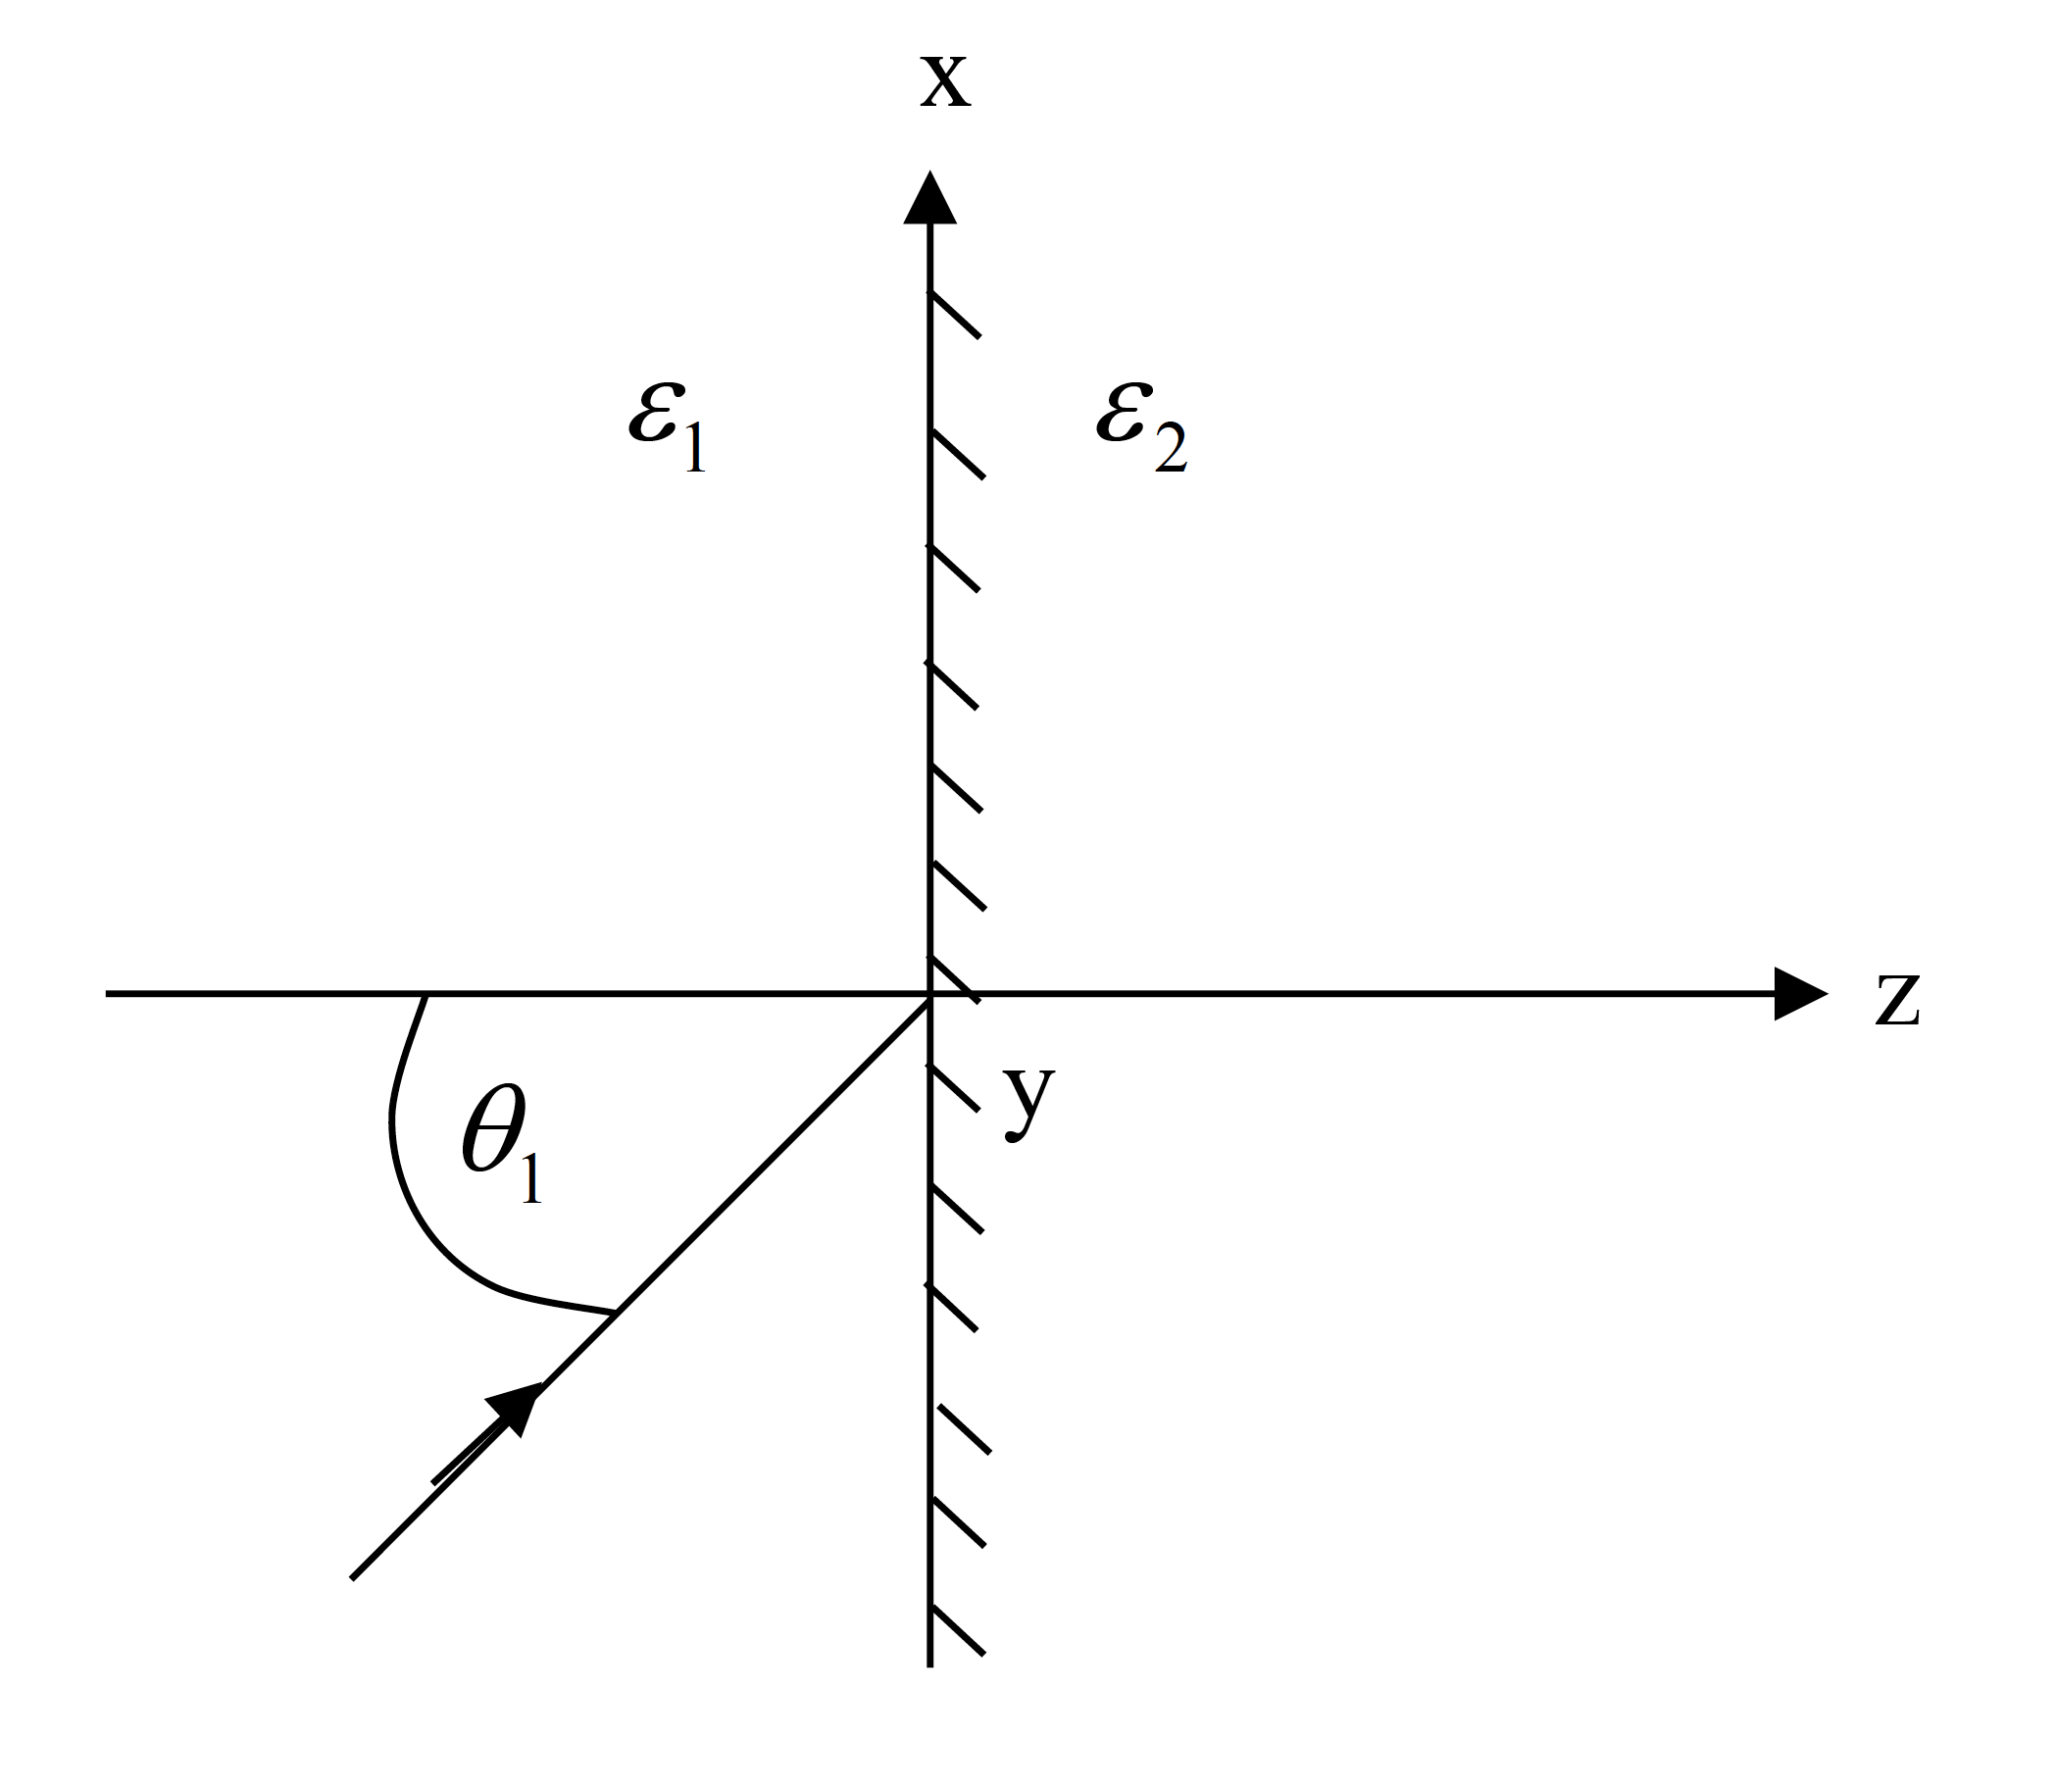
\includegraphics[width=2.0in]{figures/2018s/12q_a.png}}
\caption{Plane wave incident incident in the interface between two dielectrics}
\label{fig:12q_a}
\end{figure}

    \begin{enumerate}
        \item Find the angle $\theta_{1c}$ such that all waves incident with $\theta_1 > \theta_{1c}$ are "totally reflected".
        \item For $\theta_1 > \theta_{1c}$, describe the field (if any) in the region $z > 0$ in the $\varepsilon_2$ dielectric.
        \item If \underline{$E$} is perpendicular to the plane of the incidence, $\underline{E} = E_y \hat{y}$, find the phase of the reflection coefficient.
    \end{enumerate}

\end{enumerate}
\end{document}